\begin{name}
	{\tenchude}
	{ĐỀ ÔN TẬP CHƯƠNG I}
	{LỚP TOÁN THẦY PHÁT}
	{\thoigian}
\end{name}
\TN
\Opensolutionfile{ans}[ans/ans\currfilebase-Phan-I]
\begin{ex}%[2-D1B5-SO-13-2425]%[VN-MT-7, Lê Hải Phụng]%[2D1N1-2]
Cho hàm số $y=f(x)$ có bảng biến thiên như sau:
\begin{center}

\begin{tikzpicture}
\tkzTabInit[nocadre=true,lgt=1.2,espcl=2.5,deltacl=0.5]
{$x$/0.7,$f'(x)$/0.7,$f(x)$/2}
{$-\infty$,$-1$,$0$,$1$,$+\infty$}
\tkzTabLine{,-,0,+,0,-,0,+,}
\tkzTabVar{+/$+\infty$,-/$-1$,+/$4$,-/$-1$,+/$+\infty$}
\end{tikzpicture}
\end{center}
Hàm số đã cho đồng biến trên khoảng nào dưới đây?
\choice
{$(-\infty;-1)$}
{$(-1;1)$}
{$(0;1)$}
{\True $(-1;0)$}

\loigiai{
Dựa vào bảng biến thiên, ta thấy hàm số đã cho đồng biến trên $(-1;0)$ và $(1;+\infty)$
}
\end{ex}

\begin{ex}%[2-D1B5-SO-13-2425]%[VN-MT-7, Lê Hải Phụng]%%[2D1N2-2]
 Cho hàm số $f(x)$ có bảng biến thiên như sau:
 \begin{center}
 
\begin{tikzpicture}
 \tkzTabInit[nocadre=true,lgt=1,espcl=3,deltacl=0.5]
 {$x$/0.7,$y'$/0.7,$y$/2}
 {$-\infty$,$1$,$3$,$+\infty$}
 \tkzTabLine{,+,0,-,0,+,} 
 \tkzTabVar{-/$-\infty$,+/$3$,-/$-2$,+/$+\infty$}
 \end{tikzpicture}
 \end{center}
 Hàm số $f(x)$ đạt cực đại tại 
 \choice
 {$x=-2$}
 {$x=3$}
 {\True $x=1$}
 {$x=2$}
 
 \loigiai{
 Hàm số $f(x)$ đạt cực đại tại $x=1$.
 }
\end{ex}

\begin{ex}%[2-D1B5-SO-13-2425]%[VN-MT-7, Lê Hải Phụng]%[2D1H5-1]
 Hàm số $y = f(x)$ có bảng biến thiên như sau:
 \begin{center}
 
\begin{tikzpicture}
 \tkzTabInit[nocadre=true,lgt=1,espcl=3,deltacl=0.5]
 {$x$/0.7,$y'$/0.7,$y$/2}{$-\infty$,$1$,$+\infty$}
 \tkzTabLine{,+,d,+,}
 \tkzTabVar{-/$2$,+D-/$+\infty$/$-\infty$,+/$2$}
 \end{tikzpicture}
 \end{center}
 Hàm số đồng biến trên
 \choice
 {\True $(1;+\infty)$}
 {$(-\infty;2)$}
 {$\mathbb{R}$}
 {$\mathbb{R} \setminus \{1\}$}
 \loigiai{
 Dựa vào bảng biến thiên và bốn đáp án, hàm số đồng biến chỉ đúng với đáp án là khoảng $(1;+\infty)$.
 }
\end{ex}

\begin{ex}%[2-D1B5-SO-13-2425]%[VN-MT-7, Lê Hải Phụng]%[2D1N3-2]
 Giá trị lớn nhất của hàm số $y=x+\dfrac{4}{x}$ trên $(-4;0)$ là
 \choice
 {\True $-4$}
 {$4$}
 {$-5$}
 {$5$}
 \loigiai{Tập xác định $\mathscr{D}=\mathbb{R}\setminus \{0\}$.\\
 Đạo hàm $y'=1-\dfrac{4}{x^2}=\dfrac{x^2-4}{x^2}$.\\
 Xét $y'=0\Leftrightarrow \dfrac{x^2-4}{x^2}=0\Leftrightarrow x^2-4=0\Leftrightarrow\hoac{&x=2\\&x=-2.}$\\
 Suy ra $x=-2$ vì $x\in (-4;0)$.\\
 Ta có $y(-2)=-4$.
\begin{center}
 
\begin{tikzpicture}
 \tkzTabInit[nocadre=true,lgt=1.2,espcl=2.5,deltacl=0.5]
 {$x$/0.7,$y'$/0.7,$y$/2}
 {$-4$,$-2$,$0$}
 \tkzTabLine{,+,0,-,d,}
 \tkzTabVar{-/$-5$,+/$-4$,-D/$-\infty$}
 \end{tikzpicture}
 \end{center}
 Vậy giá trị lớn nhất của hàm số $y=x+\dfrac{4}{x}$ trên $(-4;0)$ là $-4$.}
\end{ex}

\begin{ex}%[2-D1B5-SO-13-2425]%[VN-MT-7, Lê Hải Phụng]%[2D1H3-1]
\immini{ Cho hàm số $f(x)$ có đồ thị trên $[-3;3]$ như hình vẽ.
 Giá trị lớn nhất $M$ và giá trị nhỏ nhất $m$ của hàm số $f(x)$ trên $[-3;3]$ lần lượt là
 \choice[2]
 {$M=3$; $m=-1$}
 {\True $M=4$; $m=-2$}
 {$M=3$; $m=-3$}
 {$M=-1$; $m=1$}
 }{ \begin{tikzpicture}[scale=0.7, font=\normalsize, line join=round, line cap=round,>=stealth]
 \def\xmin{-4} \def\xmax{4}
 \def\ymin{-3} \def\ymax{5}
 \draw[->] (\xmin,0)--(0,0)node[above right]{$O$}--(\xmax,0)node[below]{$x$};
 \draw[->] (0,\ymin)--(0,\ymax) node [left]{$y$};
 \clip (\xmin+0.1,\ymin+0.1) rectangle (\xmax-0.1,\ymax-0.1);
 \draw[smooth,samples=100]plot[domain=-3:-1](\x,{-1.25*(\x)^2-2.5*(\x)+1.75});
 \draw[smooth,samples=100]plot[domain=-1:1](\x,{-2*(\x)^3+1});
 \draw[smooth,samples=100]plot[domain=1:3](\x,{-3.5+2.5*(\x)});
 \draw[dashed] (-3,0)--(-3,-2)--(0,-2) (-1,0)--(-1,3)--(0,3) (0,-1)--(1,-1)--(1,0) (3,0)--(3,4)--(0,4);
 \path 
 (-3,0) node[below left]{$-3$}
 (-1,0) node[below]{$-1$}
 (1,0) node[above]{$1$}
 (3,0) node[below]{$3$}
 (0,-2) node[right]{$-2$}
 (0,-1) node[left]{$-1$}
 (0,3) node[right]{$3$}
 (0,4) node[left]{$4$};
 \fill (-3,-2) circle (1pt);
 \fill (-1,3) circle (1pt);
 \fill (1,-1) circle (1pt);
 \fill (3,4) circle (1pt);
 \end{tikzpicture}}
 \loigiai{Từ đồ thị, ta có giá trị lớn nhất $M=4$ và giá trị nhỏ nhất $m=-2$ của hàm số $f(x)$ trên $[-3;3]$.}
\end{ex}

\begin{ex}%[2-D1B5-SO-13-2425]%[VN-MT-7, Lê Hải Phụng]%[2D1H4-1]
 Đồ thị hàm số $y=\dfrac{x+1}{x^2+x-2}$ có bao nhiêu đường tiệm cận đứng?
 \choice
 {$1$}
 {\True $2$}
 {$3$}
 {$4$}
 \loigiai{Ta có $y=\dfrac{x+1}{x^2+x-2}=\dfrac{x+1}{(x-1)(x+2)}$.\\
 Hàm số đã cho có tập xác định là $\mathbb{R}\setminus\{1;-2\}$.\\
 Ta có \begin{itemize}
 \item $\lim\limits_{x\to1^-}f(x)=\lim\limits_{x\to1^-}\dfrac{x+1}{(x-1)(x+2)}=-\infty$.
 \item $\lim\limits_{x\to1^+}f(x)=\lim\limits_{x\to1^-}\dfrac{x+1}{(x-1)(x+2)}=+\infty$.
 \end{itemize} 
Suy ra $x=1$ là tiệm cận đứng của đồ thị hàm số.\\
Ta có \begin{itemize}
 \item $\lim\limits_{x\to-2^-}f(x)=\lim\limits_{x\to-2^-}\dfrac{x+1}{(x-1)(x+2)}=-\infty$.
 \item $\lim\limits_{x\to-2^+}f(x)=\lim\limits_{x\to-2^-}\dfrac{x+1}{(x-1)(x+2)}=+\infty$.
\end{itemize} 
Suy ra $x=-2$ là tiệm cận đứng của đồ thị hàm số.\\
Vậy đồ thị hàm số đã cho có $2$ đường tiệm cận đứng.}
\end{ex}

\begin{ex}%[2-D1B5-SO-13-2425]%[VN-MT-7, Lê Hải Phụng]%[2D1H4-1]
 Cho hàm số $y=f(x)=\dfrac{6x^2+7x-2023}{2x^2+3x+2024}$. Đồ thị hàm số có tiệm cận ngang là
 \choice
 {\True $y=3$}
 {$y=0$}
 {$y=1$}
 {$y=2$}
 \loigiai{Tập xác định của hàm số đã cho là $\mathbb{R}$.\\
 Ta có \begin{itemize}
 \item $\lim\limits_{x\to+\infty}f(x)=\lim\limits_{x\to+\infty}\dfrac{6x^2+7x-2023}{2x^2+3x+2024}=\dfrac{6}{2}=3$.
 \item $\lim\limits_{x\to-\infty}f(x)=\lim\limits_{x\to-\infty}\dfrac{6x^2+7x-2023}{2x^2+3x+2024}=\dfrac{6}{2}=3$.
 \end{itemize} 
 Suy ra $y=3$ là tiệm cận ngang của đồ thị hàm số.}
\end{ex}

\begin{ex}%[2-D1B5-SO-13-2425]%[VN-MT-7, Lê Hải Phụng]%[2D1H4-1]
 Tiệm cận xiên của đồ thị hàm số $y=\dfrac{x^3+x^2-2x-1}{x^2-2}$ là đường thẳng có phương trình
 \choice
 {$y=2x+1$}
 {\True $y=x+1$}
 {$y=-x+1$}
 {$y=x$}
 \loigiai{Tập xác định của hàm số $\mathscr{D}=\mathbb{R}\setminus\left\lbrace \pm\sqrt{2}\right\rbrace $.\\
 Phương trình đường tiệm cận xiên có dạng $y=ax+b$.\\
 Trong đó
 \begin{itemize}
 \item $a=\lim\limits_{x\to +\infty} \dfrac{f(x)}{x}=\lim\limits_{x\to +\infty}\dfrac{x^3+x^2-2x-1}{x^3-2x}=1$.
 \item $b=\lim\limits_{x\to +\infty} \left[f(x)-ax\right]=\lim\limits_{x\to +\infty} \left(\dfrac{x^3+x^2-2x-1}{x^2-2}-x\right)=\lim\limits_{x\to +\infty}\dfrac{x^2+1}{x^2-2}=1$.
 \end{itemize}
 Ta cũng có \begin{itemize}
 \item $a=\lim\limits_{x\to -\infty} \dfrac{f(x)}{x}=\lim\limits_{x\to -\infty}\dfrac{x^3+x^2-2x-1}{x^3-2x}=1$.
 \item $b=\lim\limits_{x\to -\infty} \left[f(x)-ax\right]=\lim\limits_{x\to -\infty} \left(\dfrac{x^3+x^2-2x-1}{x^2-2}-x\right)=\lim\limits_{x\to -\infty}\dfrac{x^2+1}{x^2-2}=1$.
 \end{itemize}
 Và $\lim\limits_{x\to \pm\infty} \left[f(x)-(ax+b)\right]=\lim\limits_{x\to \pm\infty} \left[\dfrac{x^3+x^2-2x-1}{x^2-2}-(x+1)\right]=0$.\\
 Do đó, đồ thị hàm số có tiệm cận xiên là đường thẳng $y=x+1$. }
\end{ex}

\begin{ex}%[2-D1B5-SO-13-2425]%[VN-MT-7, Lê Hải Phụng]%[2D1H5-1]
\immini{Đồ thị của hàm số nào dưới đây có dạng như đường cong trong hình bên?
 \choice[2]
 {\True $y=x^3-2024x$}
 {$y=-x^3+3x$}
 {$y=x^3-3x^2+2024$}
 {$y=-x^3+3x^2-2$}
}{ 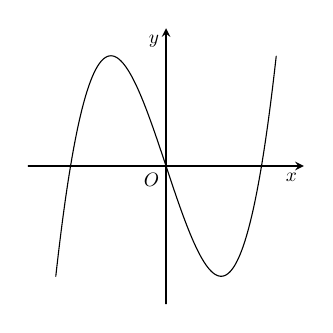
\begin{tikzpicture}[scale=0.7, line join=round, line cap=round,>=stealth]
 \tikzset{every node/.style={scale=0.7}}
 \draw[->] (-2.5,0)--(2.5,0) node[below left] {$x$};
 \draw[->] (0,-2.5)--(0,2.5) node[below left] {$y$};
 \draw (0,0) node [below left] {$O$};
 \fill (0,0) circle (1pt);
 \begin{scope}
 \clip (-2.5,-2.5) rectangle (2.5,2.5);
 \draw[samples=200,domain=-2:2,smooth,variable=\x] plot (\x,{1*((\x)^3)+0*((\x)^2)+-3*(\x)+0});
 \end{scope}
\end{tikzpicture} }
 \loigiai{Đường cong có dạng của đồ thị hàm số bậc ba với hệ số $a>0$ và đi qua $O(0;0)$. Do đó đồ thị trên của hàm số $y=x^3-2024x$.}
\end{ex}

\begin{ex}%[2-D1B5-SO-13-2425]%[VN-MT-7, Lê Hải Phụng]%[2D1H5-1]
 \immini{Cho hàm số $y=\dfrac{ax+b}{cx+d}$ có đồ thị là đường cong trong hình vẽ bên. Tọa độ giao điểm của đồ thị
 hàm số đã cho và trục tung là
 \choice[2]
 {\True $(0;-2)$}
 {$(2;0)$}
 {$(-2;0)$}
 {$(0;2)$}
 }{ \begin{tikzpicture}[scale=.5, font=\normalsize, line join=round, line cap=round,>=stealth]
 \def\xmin{-7} \def\xmax{6}
 \def\ymin{-5} \def\ymax{6}
 \draw[->] (\xmin,0)--(0,0)node[below left]{$O$}--(\xmax,0)node[below]{$x$};
 \draw[->] (0,\ymin)--(0,\ymax) node [left]{$y$};
 \clip (\xmin+0.1,\ymin+0.1) rectangle (\xmax-0.1,\ymax-0.1);
 \draw[smooth,samples=100]plot[domain=\xmin:\xmax](\x,{(\x-2)/(\x+1)}) (\xmin,1)--(\xmax,1);
 \path 
 (-1,0) node[below left]{$-1$}
 (2,0) node[below]{$2$}
 (0,1) node[above right]{$1$}
 (0,-2) node[right]{$-2$};
 \fill (0,0) circle (1pt);
 \fill (-1,1) circle (1pt);
 \fill (0,1) circle (1pt);
 \fill (-1,0) circle (1pt);
 \fill (2,0) circle (1pt);
 \fill (0,-2) circle (1pt);
 \end{tikzpicture}}
 \loigiai{Từ đồ thị hàm số đã cho, ta có tọa độ giao điểm của đồ thị hàm số đã cho và trục tung là $(0;-2)$.}
\end{ex}

\begin{ex}%[2-D1B5-SO-13-2425]%[VN-MT-7, Lê Hải Phụng]%[2D1H5-1]
 \immini{Đồ thị của hàm số nào dưới đây có dạng như đường cong trong hình bên dưới?
 \choice
 {$y=x+2$}
 {$y=\dfrac{x^2-2x+2}{x+1}$}
 {$y=x^2-2x+2$}
 {\True $\dfrac{x^2+2x+2}{x+1}$}
 }{ 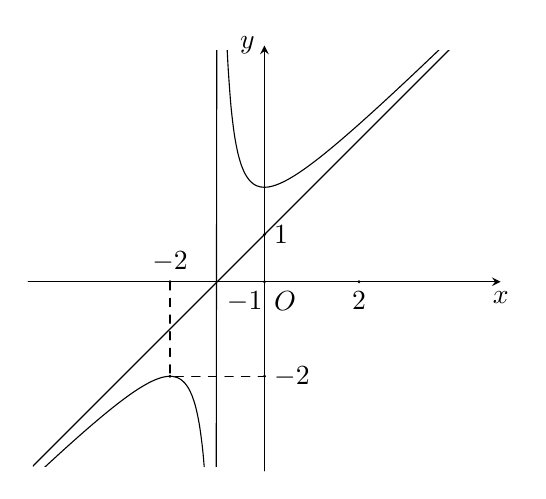
\begin{tikzpicture}[scale=.6, font=\normalsize, line join=round, line cap=round,>=stealth]
 \def\xmin{-5} \def\xmax{5}
 \def\ymin{-4} \def\ymax{5}
 \draw[->] (\xmin,0)--(0,0)node[below right]{$O$}--(\xmax,0)node[below]{$x$};
 \draw[->] (0,\ymin)--(0,\ymax) node [left]{$y$};
 \clip (\xmin+0.1,\ymin+0.1) rectangle (\xmax-0.1,\ymax-0.1);
 \draw[smooth,samples=125]plot[domain=\xmin:\xmax](\x,{((\x)^2+2*(\x)+2)/(\x+1)});
 \draw[smooth,samples=125]plot[domain=\xmin:\xmax](\x,{(\x)+1});
 \draw[dashed] (-2,0)--(-2,-2)--(0,-2);
 \path 
 (-1,0) node[below right]{$-1$}
 (2,0) node[below]{$2$}
 (-2,0) node[above]{$-2$}
 (0,1) node[right]{$1$}
 (0,-2) node[right]{$-2$};
 \fill (0,0) circle (1pt);
 \fill (0,1) circle (1pt);
 \fill (0,-2) circle (1pt);
 \fill (2,0) circle (1pt);
 \fill (-2,0) circle (1pt);
 \fill (-2,-2) circle (1pt);
 \end{tikzpicture}}
 \loigiai{Từ đồ thị ta thấy $x=-1$ là tiệm cận đứng của đồ thị hàm số đã cho và đi qua $(-2;-2)$.\\
 Vậy đồ thị trên của hàm số $y=\dfrac{x^2+2x+2}{x+1}$.}
\end{ex}

\begin{ex}%[2-D1B5-SO-13-2425]%[VN-MT-7, Lê Hải Phụng]%[2D1H5-1]
 \immini{Cho hàm số $y=\dfrac{x^2+a}{x+b}$ có đồ thị là đường cong trong hình vẽ bên. Giá trị của $T=a+b$ bằng
 \choice
 {$T=0$}
 {$T=-2$}
 {\True $T=-1$}
 {$T=2$}
 }{ 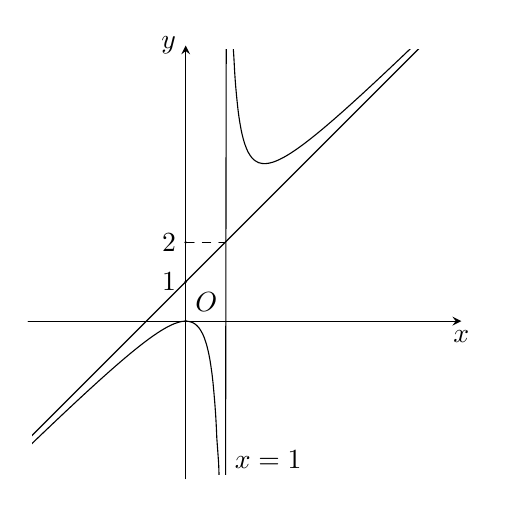
\begin{tikzpicture}[scale=.5, font=\normalsize, line join=round, line cap=round,>=stealth]
 \def\xmin{-4} \def\xmax{7}
 \def\ymin{-4} \def\ymax{7}
 \draw[->] (\xmin,0)--(0,0)node[above right]{$O$}--(\xmax,0)node[below]{$x$};
 \draw[->] (0,\ymin)--(0,\ymax) node [left]{$y$};
 \clip (\xmin+0.1,\ymin+0.1) rectangle (\xmax-0.1,\ymax-0.1);
 \draw[smooth,samples=125]plot[domain=\xmin:\xmax](\x,{((\x)^2)/(\x-1)});
 \draw[smooth,samples=100]plot[domain=\xmin:\xmax](\x,{(\x)+1});
 \draw[dashed] (0,2)--(1,2);
 \path 
 (0,1) node[left]{$1$}
 (0,2) node[left]{$2$}
 (1,\ymin) node[above right]{$x=1$};
 \fill (0,0) circle (1pt);
 \fill (0,1) circle (1pt);
 \fill (0,2) circle (1pt);
 \end{tikzpicture}}
 \loigiai{Từ đồ thị ta thấy $x=1$ là tiệm cận đứng của đồ thị hàm số nên $b=-1$. Suy ra $y=\dfrac{x^2+a}{x-1}$.\\
 Hàm số đi qua $(0;0)$ nên $\dfrac{0^2+a}{0-1}=0\Leftrightarrow a=0$.\\
 Vậy $T=a+b=0+(-1)=-1$.}
\end{ex}
\Closesolutionfile{ans}

\TNTF
\Opensolutionfile{ans}[ans/ans\currfilebase-Phan-II]
\begin{ex}%[2-D1B5-SO-13-2425]%[VN-MT-7, Lê Hải Phụng]%[2D1H2-1]
Cho hàm số $y=f(x)=x^4-2x^2-5$. Các khẳng định sau là đúng hay sai?
\choiceTF
{\True Hàm số có $3$ điểm cực trị}
{Hàm số đồng biến trên $(0;+\infty)$}
{Điểm $M(0;1)$ là điểm cực đại của đồ thị hàm số $y=f(x)$}
{Hàm số $y=f(x)$ và $y=f(2x)$ có cùng điểm cực đại}
\loigiai{
 Tập xác định $\mathscr{D}=\mathbb{R}$.\\
 Đạo hàm $y'=4x^3-4x$.\\
 Xét $y'=0\Leftrightarrow 4x^3-4x=0\Leftrightarrow\hoac{&x=0\\&x=1\\&x=-1.}$\\
 Bảng biến thiên
 \begin{center}
 
\begin{tikzpicture}
 \tkzTabInit[nocadre=true,lgt=1.2,espcl=2.5,deltacl=0.5]
 {$x$/0.7,$f'(x)$/0.7,$f(x)$/2}
 {$-\infty$,$-1$,$0$,$1$,$+\infty$}
 \tkzTabLine{,-,0,+,0,-,0,+,}
 \tkzTabVar{+/$+\infty$,-/$-6$,+/$-5$,-/$-6$,+/$+\infty$}
 \end{tikzpicture}
 \end{center}
\begin{itemchoice}
\itemch \textbf{Đúng}.\\
Hàm số có $3$ điểm cực trị là $x=-1$, $x=0$, $x=1$.
\itemch \textbf{Sai}.\\
Hàm số đồng biến trên $(-1;0)$ và $(1;+\infty)$.
\itemch \textbf{Sai}.\\
Điểm $M(0;-5)$ là điểm cực đại của đồ thị hàm số $y=f(x)$
\itemch \textbf{Đúng}.\\
Xét $y=f(2x)$, ta có $y'=2f'(2x)$.\\
Xét $y'=0\Leftrightarrow 2f'(2x)=0\Leftrightarrow f'(2x)=0\Leftrightarrow \hoac{&2x=-1\\&2x=0\\&2x=1}\Leftrightarrow\hoac{&x=-\dfrac{1}{2}\\&x=0\\&x=\dfrac{1}{2}.}$\\
Bảng biến thiên
\begin{center}
 
\begin{tikzpicture}
 \tkzTabInit[nocadre=true,lgt=1.2,espcl=2.5,deltacl=0.5]
 {$x$/0.7,$y'$/0.7,$y$/2}
 {$-\infty$,$-\tfrac{1}{2}$,$0$,$\tfrac{1}{2}$,$+\infty$}
 \tkzTabLine{,-,0,+,0,-,0,+,}
 \tkzTabVar{+/$+\infty$,-/$f(-1)$,+/$f(0)$,-/$f(1)$,+/$+\infty$}
 \end{tikzpicture}
\end{center}
Suy ra $x=0$ là điểm cực đại của hàm số $y=f(2x)$.\\
Vậy hàm số $y=f(x)$ và $y=f(2x)$ có cùng điểm cực đại.
\end{itemchoice}
}
\end{ex}

\begin{ex}%[2-D1B5-SO-13-2425]%[VN-MT-7, Lê Hải Phụng]%[2D1H3-1]
 Cho hàm số $y=f(x)=x^3-3x+2$. Các khẳng định sau là đúng hay sai?
 \choiceTF
 {\True $\min\limits_{[0;1]} y=0$}
 {\True $\min\limits_{[0;2]} y=y(0)$}
 {$\min\limits_{[-1;0]} y+\max\limits_{[0;1]} y=4$}
 {$\min\limits_{\left[-\frac{3}{2};0 \right] } \dfrac{1}{y}=\dfrac{8}{25}$}
 \loigiai{ Tập xác định $\mathscr{D}=\mathbb{R}$.\\
 Đạo hàm $y'=3x^2-3$.\\
 Xét $y'=0\Leftrightarrow 3x^2-3=0\Leftrightarrow\hoac{&x=1\\&x=-1.}$\\
 Bảng biến thiên
 \begin{center}
 
\begin{tikzpicture}
 \tkzTabInit[nocadre=true,lgt=1.2,espcl=2.5,deltacl=0.5]
 {$x$/0.7,$f'(x)$/0.7,$f(x)$/2}
 {$-\infty$,$-1$,$1$,$+\infty$}
 \tkzTabLine{,+,0,-,0,+,}
 \tkzTabVar{-/$+\infty$,+/$4$,-/$0$,+/$-\infty$}
 \end{tikzpicture}
 \end{center}
 \begin{itemchoice}
 \itemch \textbf{Đúng}.\\
 Ta xét trên $[0;1]$, ta có $y(0)=2$ và $y(1)=0$. Vậy $\min\limits_{[0;1]} y=0$.
 \itemch \textbf{Đúng}.\\
 Ta xét trên $[0;2]$, ta có $y(0)=2$, $y(1)=0$ và $y(2)=4$. Vậy $\min\limits_{[0;2]} y=0=y(0)$.
 \itemch \textbf{Sai}.\\
 Ta xét trên $[0;1]$, ta có $y(0)=2$ và $y(1)=0$. Vậy $\min\limits_{[0;1]} y=0$ và $\max\limits_{[0;1]} y=2$, khi đó tổng bằng $0+2=2$.
 \itemch \textbf{Sai}.\\
 Ta có $g(x)=\dfrac{1}{y}=\dfrac{1}{x^3-3x+2}$.\\
 Tập xác định $\mathscr{D}=\mathbb{R}\setminus\{-2;1\}$.\\
 $g'(x)=\left(\dfrac{1}{y} \right)'=\dfrac{-3x^2-3}{x^3-3x+2}$.\\
 Bảng biến thiên
 \begin{center}
 
\begin{tikzpicture}
 \tkzTabInit[nocadre=true,lgt=1.2,espcl=2.5,deltacl=0.5]
 {$x$/0.7,$g'(x)$/0.7,$g(x)$/2}
 {$-\tfrac{3}{2}$,$-1$,$0$}
 \tkzTabLine{,-,0,+,}
 \tkzTabVar{+/$\dfrac{8}{25}$,-/$\dfrac{1}{4}$,+/$\dfrac{1}{2}$}
 \end{tikzpicture}
 \end{center}
 Vậy $\min\limits_{\left[-\frac{3}{2};0 \right] } \dfrac{1}{y}=\dfrac{1}{4}$ khi $x=-1$.
 \end{itemchoice}
 }
\end{ex}

\begin{ex}%[2-D1B5-SO-13-2425]%[VN-MT-7, Lê Hải Phụng]%[2D1H4-1]
 Hàm số $y = f(x)$ có bảng biến thiên như sau
 \begin{center}
 
\begin{tikzpicture}
 \tkzTabInit[nocadre=true,lgt=1.2,espcl=2.5,deltacl=0.5]
 {$x$/0.7,$y'$/0.7,$y$/2}{$-\infty$,$2$,$+\infty$}
 \tkzTabLine{,+,d,+,}
 \tkzTabVar{-/$1$,+D-/$+\infty$/$-\infty$,+/$1$}
 \end{tikzpicture}
 \end{center}
 \choiceTF
 {\True Tập xác định của hàm số là $\mathscr{D}=\mathbb{R}\setminus\{2\}$}
 {Hàm số đồng biến trên $\mathbb{R}$}
 {\True Tiệm cận ngang của hàm số là $y = 1$}
 {Hàm số đạt cực đại tại $x = 2$}
 \loigiai{
 \begin{itemchoice}
 \itemch \textbf{Đúng}.\\
 Tập xác định của hàm số là $\mathscr{D}=\mathbb{R}\setminus\{2\}$.
 \itemch \textbf{Sai}.\\
 Hàm số đống biến trên $(-\infty; 2)$ và $(2; +\infty)$.
 \itemch \textbf{Đúng}.\\
 Vì $\lim\limits_{x \to -\infty} f(x) = 1$ nên tiệm cận ngang của hàm số là $y = 1$.
 \itemch \textbf{Sai}.\\
 Hàm số không có cực trị.
 \end{itemchoice}
 }
\end{ex}

\begin{ex}%[2-D1B5-SO-13-2425]%[VN-MT-7, Lê Hải Phụng]%[2D1H5-7]
 \immini{
 Cho hàm số $y = f(x)$ có đồ thị như sau. Các mệnh đề sau đúng hay sai?
 \choiceTF
 {Hàm số đồng biến trên $(-\infty; -1)$}
 {Hàm số đạt cực đại tại $x = -2$}
 {\True Giá trị nhỏ nhất của hàm số $y = f(x)$ trên $(-\infty;-1)$ là $\dfrac{3}{2}$}
 {\True Điểm cực tiểu của hàm số là $x = -2$}}{ \begin{tikzpicture}[scale=0.7, font=\footnotesize, line join=round, line cap=round, >=stealth]
 \def \a{1}
 \def \b{1}
 \def \c{1}
 \def \u{-2}
 \def \v{-2}
 \def \f{((\a)*(\x)^2+(\b)*(\x)+(\c))/((\u)*(\x)+(\v))} %%Hàm số
 \def \tcx{-(\x)/2} %Tiệm cận xiên
 \def \xo{-{\v/\u}} %Tiệm cận đứng
 \def \yo{0.5} %Tiệm cận ngang
 \def \kx{4.5} %độ rộng của đồ thị theo x
 \draw[->] (\xo-\kx,0)--(\xo+\kx,0) node[below left] {$x$};
 \draw[->] (0,\yo-\kx)--(0,\yo+\kx) node[below left] {$y$};
 \draw (0,0) node [above right] {\scriptsize $O$};
 \draw[dashed] (-1,1pt)--(-1,-1pt) + (-30:6mm) node {\scriptsize $-1$};
 \draw[dashed] (-2,1pt)--(-2,-1pt) + (-90:6mm) node {\scriptsize $-2$};
 \draw[dashed] (1pt,1.5)--(-1pt,1.5) + (0:6mm) node {\scriptsize $\dfrac{3}{2}$};
 \draw[dashed] (1pt,-0.5)--(-1pt,-0.5) + (-45:10mm) node {\scriptsize $-\dfrac{1}{2}$};
 \begin{scope}
 \clip (\xo-\kx,\yo-\kx) rectangle (\xo+\kx,\yo+\kx);
 \draw[smooth,samples=200,domain=\xo-\kx:\xo-0.1,smooth,variable=\x] plot (\x,{\f});
 \draw[smooth,samples=200,domain=\xo+0.1:\xo+\kx,smooth,variable=\x] plot (\x,{\f});
 %Tiệm cận
 \draw[thin] (\xo,\yo-\kx)--(\xo,\yo+\kx);
 \draw[smooth,samples=200,domain=\xo-\kx:\xo+\kx,variable=\x] plot (\x,{\tcx});
 \end{scope}
 %Vẽ đường dóng
 \draw[dashed, thin] (-2,0) -- (-2,1.5) -- (0,1.5);
 \fill (0,0) circle (1pt);
 \fill (-2,0) circle (1pt);
 \fill (-1,0) circle (1pt);
 \fill (0,-0.5) circle (1pt);
 \fill (0,1.5) circle (1pt);
 \fill (-2,1.5) circle (1pt); 
 \end{tikzpicture}}
 \loigiai{
 \begin{itemchoice}
 \itemch \textbf{Sai}.\\
 Hàm số đồng biến trên $(-2;-1)$, $(-1;0)$ và nghịch biến trên $(-\infty;-2)$, $(0;+\infty)$.
 \itemch \textbf{Sai}.\\
 Hàm số đạt cực tiểu tại $x = -2$.
 \itemch \textbf{Đúng}.\\
 Giá trị nhỏ nhất của hàm số $y = f(x)$ trên $(-\infty;-1)$ là $\dfrac{3}{2}$.
 \itemch \textbf{Đúng}.\\
 Điểm cực tiểu của hàm số là $x = -2$.
 \end{itemchoice}
 }
\end{ex}
\Closesolutionfile{ans}

\TNSA
\Opensolutionfile{ans}[ans/ans\currfilebase-Phan-III]
\begin{ex}%[2-D1B5-SO-13-2425]%[VN-MT-7, Lê Hải Phụng]%[2D1N1-1]
 Cho hàm số $y=x^3-3x^2+1$. Tính tổng của tất cả các giá trị cực đại và giá trị cực tiểu của hàm số trên. 
 
 \shortans{-2}
 
 \loigiai{Tập xác định của hàm số $\mathscr{D}=\mathbb{R}$.\\
 Ta có đạo hàm $y'=3x^2-6x$.\\
 Xét $y'=0\Leftrightarrow3x^2-6x=0\Leftrightarrow\hoac{&x=0\\&x=2.}$\\
 Bảng biến thiên:\\
 \begin{center}
 
\begin{tikzpicture}
 \tkzTabInit[nocadre=true,lgt=1,espcl=3,deltacl=0.5]
 {$x$/0.7,$y'$/0.7,$y$/2}
 {$-\infty$,$0$,$2$,$+\infty$}
 \tkzTabLine{,+,0,-,0,+,} 
 \tkzTabVar{-/$-\infty$,+/$1$,-/$-3$,+/$+\infty$}
 \end{tikzpicture}
 \end{center}
 Suy ra giá trị cực đại và cực tiểu lần lượt là $y=1$ và $y=-3$. Khi đó $1+(-3)=-2$.}
\end{ex}

\begin{ex}%[2-D1B5-SO-13-2425]%[VN-MT-7, Lê Hải Phụng]%[2D1H4-1]
 Tiệm cận xiên của đồ thị hàm số $y=f(x)=\dfrac{3x-x^2}{2x-1}$ là đường thẳng $y=ax+b$. Tính giá trị của biểu thức $P=a^2-b$.
 
 \shortans{-1}
 
 \loigiai{Tập xác định của hàm số $\mathscr{D}=\mathbb{R}\setminus\left\lbrace \dfrac{1}{2}\right\rbrace $.\\
 Phương trình đường tiệm cận xiên có dạng $y=ax+b$.\\
 Trong đó
 \begin{itemize}
 \item $a=\lim\limits_{x\to +\infty} \dfrac{f(x)}{x}=\lim\limits_{x\to +\infty}\dfrac{3x-x^2}{2x^2-x}=-\dfrac{1}{2}$.
 \item $b=\lim\limits_{x\to +\infty} \left[f(x)-ax\right]=\lim\limits_{x\to +\infty} \left(\dfrac{3x-x^2}{2x-1}+\dfrac{1}{2}x\right)=\dfrac{5}{4}$.
 \end{itemize}
 Ta cũng có \begin{itemize}
 \item $a=\lim\limits_{x\to -\infty} \dfrac{f(x)}{x}=\lim\limits_{x\to -\infty}\dfrac{3x-x^2}{2x^2-x}=-\dfrac{1}{2}$.
 \item $b=\lim\limits_{x\to -\infty} \left[f(x)-ax\right]=\lim\limits_{x\to -\infty} \left(\dfrac{3x-x^2}{2x-1}+\dfrac{1}{2}x\right)=\dfrac{5}{4}$.
 \end{itemize}
 Và $\lim\limits_{x\to \pm\infty} \left[f(x)-(ax+b)\right]=\lim\limits_{x\to \pm\infty} \left[\dfrac{3x-x^2}{2x-1}-\left(-\dfrac{1}{2}x+\dfrac{5}{4} \right) \right]=0$.\\
 Do đó, đồ thị hàm số có tiệm cận xiên là đường thẳng $y=-\dfrac{1}{2}x+\dfrac{5}{4}$.\\
 Do đó $a=-\dfrac{1}{2}$ và $b=\dfrac{5}{4}$. Vậy $P=-1$.}
\end{ex}

\begin{ex}%[2-D1B5-SO-13-2425]%[VN-MT-7, Lê Hải Phụng]%[2D1N5-4]
 Hàm số $y=f(x)=-x^3+2x^2-x+1$ có đồ thị $(C)$ và hàm số $y=g(x)=1$ có đồ thị là $(d)$. Số giao điểm của $(C)$ và $(d)$ là
 
 \shortans{2}
 \loigiai{Ta xét phương trình hoành độ giao điểm:
 \[-x^3+2x^2-x+1=1\Leftrightarrow-x^3+2x^2-x=0\Leftrightarrow\hoac{&x=0\\&x=1.}\]
 Suy ra giao điểm của $(C)$ và $(d)$ là $(0;1)$ và $(1;1)$.\\
 Vậy số giao điểm của $(C)$ và $(d)$ là $2$.}
\end{ex}

\begin{ex}%[2-D1B5-SO-13-2425]%[VN-MT-7, Lê Hải Phụng]%[2D1V2-7]
 Giả sử doanh số (tính bằng sản phẩm) của một sản phẩm mới (trong một năm nhất định) tuân theo quy luật logistic được mô hình hóa bằng hàm số \[f(t)=\dfrac{5000}{1+5\mathrm{e}^{-t}},\, t\ge0,\]
 trong đó thời gian $t$ được tính bằng năm, kể từ khi phát hành sản phẩm mới. Khi đó đạo hàm $f'(t)$ biểu thị tốc độ bán hàng. Hỏi sau khi phát hành bao nhiêu năm thì tốc độ bán hàng là cực đại? (làm tròn đến chữ số thập phân thứ nhất)
 
 \shortans{1{,}6}
 
 \loigiai{
 Gọi $g(t)$ là hàm tốc độ bán hàng.\\
 Khi đó $g(t)=f'(t)=\dfrac{25\,000\mathrm{e}^{-t}}{(1+5\mathrm{e}^{-t})^2}$, $t\ge0$.\\
 Ta có $g'(t)=\dfrac{25\,000\mathrm{e}^{-t}(1+5\mathrm{e}^{-t})(5\mathrm{e}^{-t}-1)}{(1+5\mathrm{e}^{-t})^4}$; $g'(t)=0\Leftrightarrow t=-\ln{\dfrac{1}{5}}$.\\
 Bảng biến thiên hàm số
 \begin{center}
 
\begin{tikzpicture}
 \tkzTabInit[nocadre=true,lgt=1.3,espcl=2.5,deltacl=0.6]
 {$t$ /0.6, $g'(t)$ /0.6, $g(t)$ /2.5}
 {$0$, $-\ln{\tfrac{1}{5}}$, $+\infty$}
 \tkzTabLine{,+,0,-,}
 \tkzTabVar{-/ $694{,}4$,+/$1250$,-/$0$}
 \end{tikzpicture}
 \end{center}
 Hàm số đạt cực đại tại $t=-\ln{\dfrac{1}{5}}\approx1{,}6$.\\
 Vậy sau khi phát hành $1{,}6$ năm thì tốc độ bán hàng là cực đại.
 }
\end{ex}

\begin{ex}%[2-D1B5-SO-13-2425]%[VN-MT-7, Lê Hải Phụng]%[2D1C5-8]
 Một tàu đổ bộ tiếp cận Mặt Trăng theo cách tiếp cận thẳng đứng và đốt cháy các tên lửa hãm ở độ cao $677{,}6$ km so với bề mặt của Mặt Trăng được tính (gần đúng) bởi hàm
 \[h(t) = 0{,}01t^3 - 1{,}16t^2 + 34{,}52t - 46{,}4\]
 Trong khoảng thời gian $t$ ở $50$ giây đầu $(0 \le t \le 50)$. Khoảng cách con tàu lớn nhất so với bề mặt của Mặt Trăng là bao nhiêu?
 
 \shortans{260}
 
 \loigiai{
 Hàm số $h(t) = 0{,}01t^3 - 1{,}16t^2 + 34{,}52t - 46{,}4$.\\
 + Tập xác định $\mathscr{D} = \mathbb{R}$.\\
 + Đạo hàm $h'(t) = 0{,}03t^2 - 2{,}32t + 34{,}52 = 0 \Leftrightarrow \hoac{&x = \dfrac{-10\sqrt{31}+116}{3} \quad\in (0;50)\\&x = \dfrac{10\sqrt{31}+116}{3} \quad \not\in (0;50).}$\\
 + $\heva{&h(0) = 34{,}52\\&h(50) = 29{,}6\\&h\left(\dfrac{-10\sqrt{31}+116}{3}\right) = 260} \Rightarrow \max\limits_{0\le t \le 50} = 260$.\\
 Vậy trong khoảng thời gian $t$ ở $50$ giây đầu $(0 \le t \le 50)$. Khoảng cách con tàu lớn nhất so với bề mặt của Mặt Trăng là $260$ km.
 }
\end{ex}

\begin{ex}%[2-D1B5-SO-13-2425]%[VN-MT-7, Lê Hải Phụng]%[2D1V3-6]
 \immini{
 Sự phân huỷ của rác thải hữu cơ có trong nước sẽ làm tiêu hao oxygen hoà tan trong nước. Nồng độ oxygen (mg/l) trong một hồ nước sau $t$ giờ $(t \geq 0)$ khi một lượng rác thải hữu cơ bị xả vào hồ được xấp xỉ bởi hàm số (có đồ thị như đường cong ở hình bên)
 \[
 y(t)=5-\dfrac{15t}{9t^2+1}.
 \]
 }{
 \begin{tikzpicture}[>=stealth,x=1cm,y=0.3cm,scale=2,font=\footnotesize]
 \draw[->] (-0.5,0) -- (4,0) node[below] {$t$};
 \draw[->] (0,-1) -- (0,6) node[left] {$y$};
 \filldraw (0,0) circle (1pt)node[below left]{$O$};
 \draw[domain=0:4,samples=200,red] plot (\x,{5-(15*(\x))/(9*(\x)^2+1)});
 \draw[dashed] (0,5) node [left] {$5$}--(4,5);
 \foreach \x/\g in {1/-90,2/-90,3/-90}
 \draw[thin] (\x,2pt)--(\x,-2pt) + (\g:3mm) node {$\x$};
 \end{tikzpicture}
 }
%  \noindent
%  (Theo: https://www.researchgate.net/publication/264903978$\_$Microrespirometric$\_$ characterization$\_$\\of$\_$activated$\_$sludge$\_$inhibition$\_$by$\_$copper$\_$and$\_$zinc)\\
 Trong đó, đạo hàm $y'(t)$ biểu thị tốc độ thay đổi nồng độ oxigen trong nước. Tốc độ thay đổi nồng độ oxigen lớn nhất khi $t=\dfrac{\sqrt{a}}{b}$ giờ. Tính giá trị của $a-b$ biết $a$ và $b$ là các số nguyên tố.
 
 \shortans{0}
 
 \loigiai{
 Ta có $y'(t)=\dfrac{135t^2-15}{(9t^2+1)^2}$.\\
 Suy ra $y''(t)=\dfrac{-2430t^3+810t}{(9t^2+1)^3}$.\\
 Cho $y''(t)=0\Leftrightarrow -2430t^3+810t=0\Leftrightarrow \hoac{&t=\pm\dfrac{\sqrt{3}}{3}\\&t=0.}$
 \begin{center}
 
\begin{tikzpicture}[>=stealth]
 \tkzTabInit[nocadre=true,lgt=1.5,espcl=3,deltacl=0.6]{$t$/1 ,$y''(t)$/.6,$y'(t)$/2}
 {$0$ , $\tfrac{\sqrt{3}}{3}$ , $+\infty$}
 \tkzTabLine{ $0$, + , $0$ , - , }
 \tkzTabVar{-/$-15$ , +/$\dfrac{15}{8}$ , -/$0$}
 \end{tikzpicture}
 \end{center}
 Từ bảng biến thiên ta có $\max\limits_{t\in[0;+\infty)}y'(t)=y'\left(\dfrac{\sqrt{3}}{3}\right)=\dfrac{15}{8}$. \\
 Vậy tốc độ thay đổi nồng độ oxigen lớn nhất khi $t=\dfrac{\sqrt{3}}{3}$ giờ.\\
 Vậy $a=b=3$. Khi đó $a-b=0$.
 }
\end{ex}
\Closesolutionfile{ans}
% \begin{indapan}
% 	{ans/ans\currfilebase}
% \end{indapan}

